\begin{figure}[p!]
\centering
\vspace{-5pt}
\subfloat[\hspace{10pt}AWS Sensor Only]{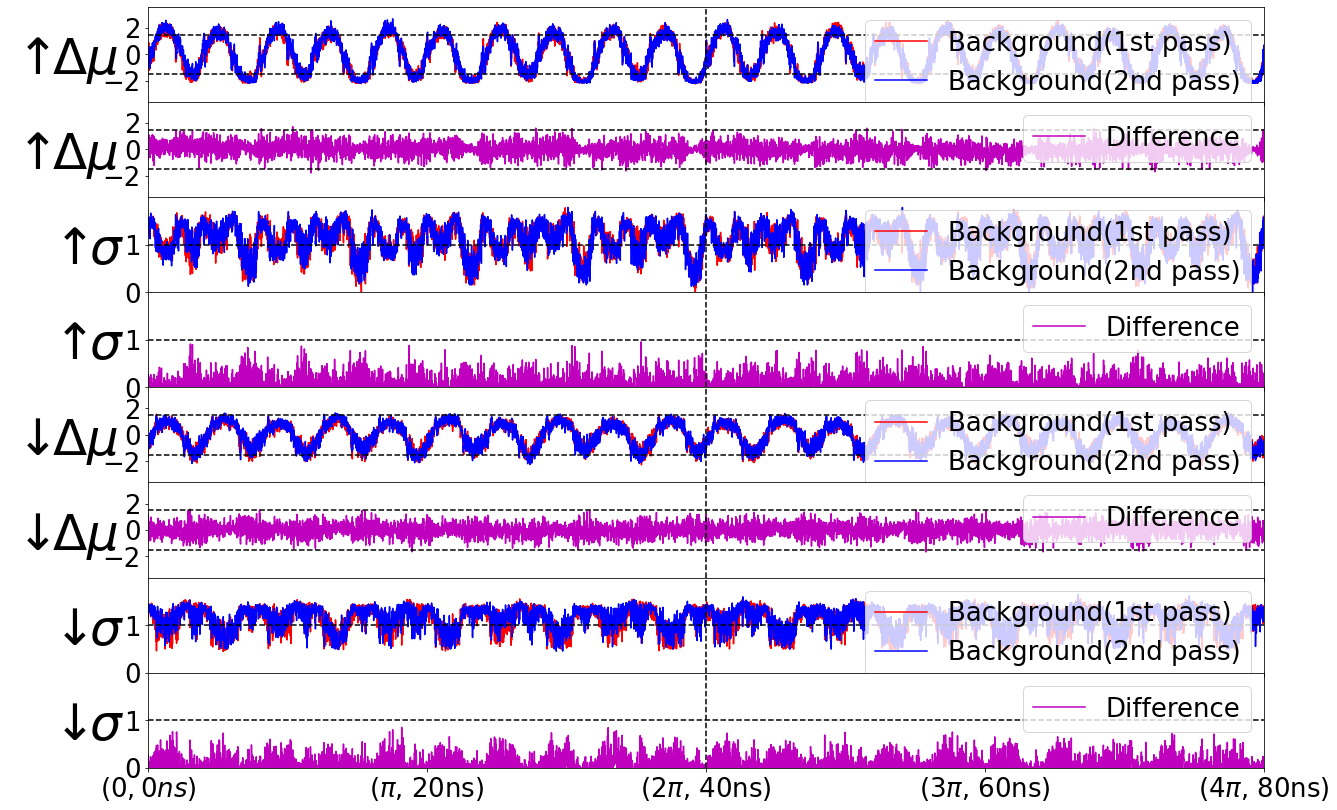
\includegraphics[width= 0.6\linewidth]{img/base_DIFF_aws_std_ham_pn_4pi.png}\label{fig:phi-aws-base}}\\
\vspace{-12px}
\subfloat[\hspace{10pt}PYNQ-Z2 Sensor Only]{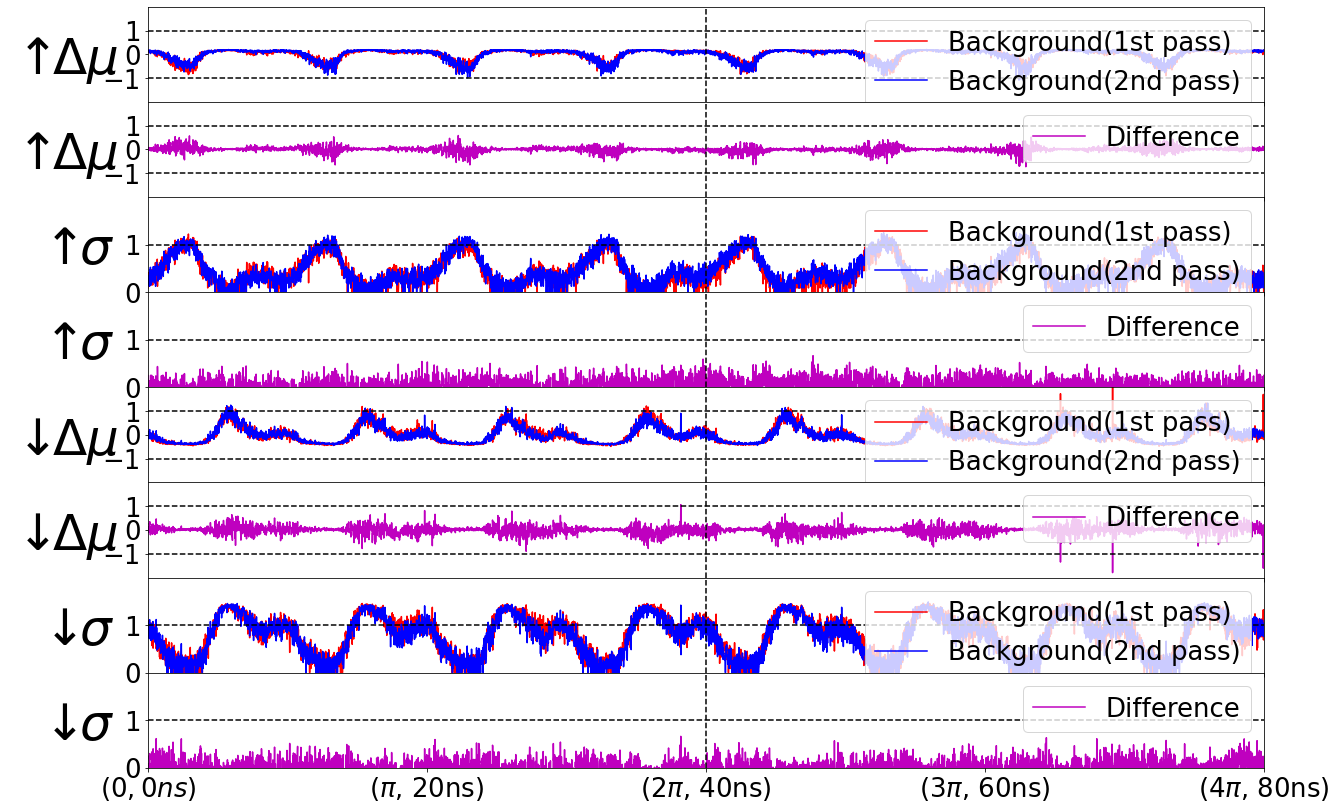
\includegraphics[width= 0.6\linewidth]{img/base_DIFF_pynq_std_ham_pn_4pi.png}\label{fig:phi-pynq-base}}\\
\vspace{-12px}
\subfloat[\hspace{10pt}PYNQ-Z2 PicoRV AES]{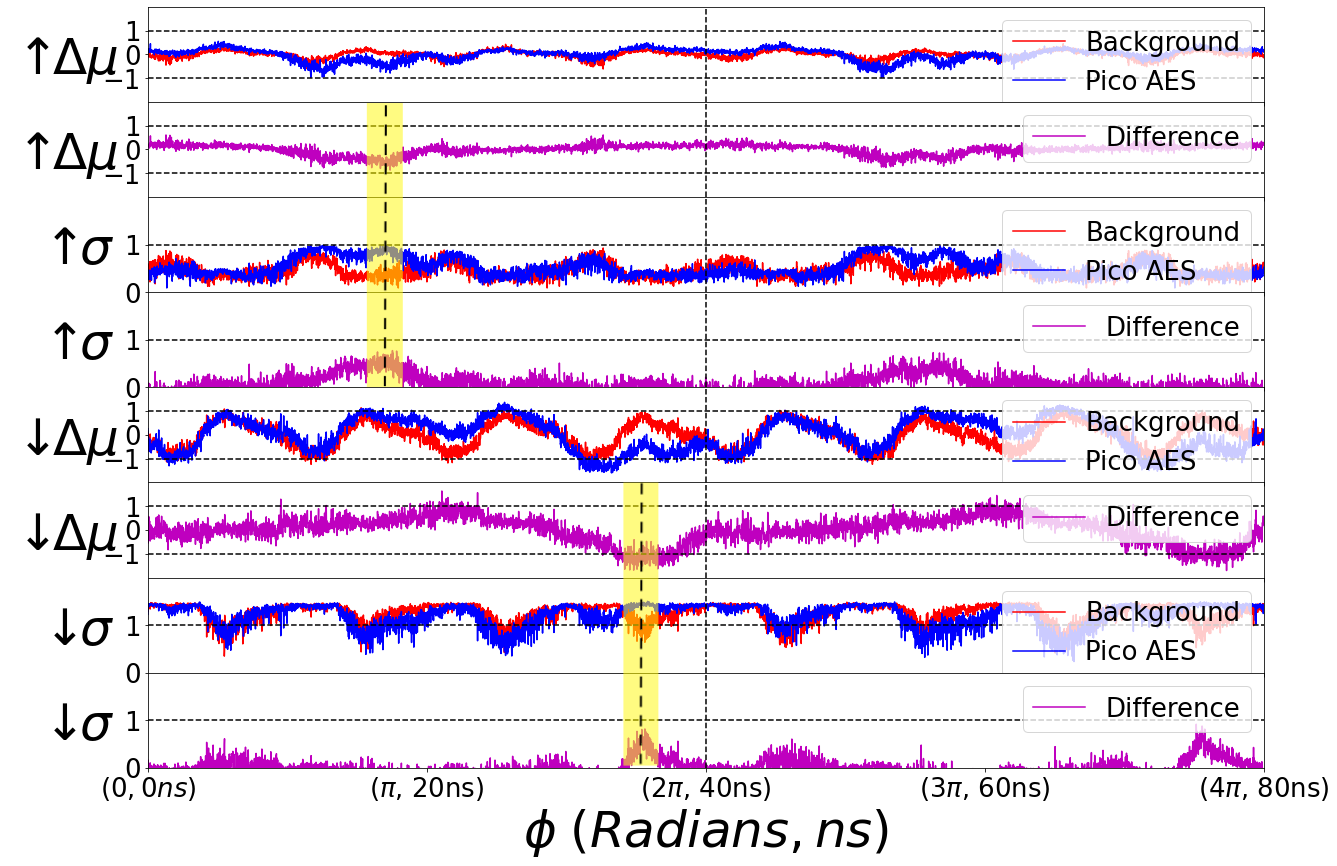
\includegraphics[width= 0.6\linewidth]{img/pico_aes_DIFF_pynq_std_ham_pn_4pi.png}\label{fig:phi-pynq-pico}}
\vspace{-12px}
\caption{Measuring sensor output as $\phi$ is swept from 0 to 4$\pi$. Background noise is consistent across multiple sweeps of $\phi$, as demonstrated rows 3 and 6 of Figure~\ref{fig:phi-aws-base} and~\ref{fig:phi-pynq-base}. Background subtraction is critical to isolate the variance caused by a target from other information sources on the system and determine the value of $\phi$ that maximizes the information leakage (yellow). The rising ($\uparrow$) and falling ($\downarrow$) transition variance maxima are offset by $\pi$. \label{fig:phi_xilinx}}
\vspace{-20px}
\end{figure} 
%Measuring sensor output as $\phi$ is swept from 0 to 4$\pi$ on the AWS Sensor Only Design. Background noise is consistent across multiple sweeps of $\phi$.

%Measuring sensor output as $\phi$ is swept from 0 to 4$\pi$ on the PYNQ-Z2 Sensor Only Design. Background noise is consistent across multiple sweeps of $\phi$.

%Measuring sensor output as $\phi$ is swept from 0 to 4$\pi$ on PYNQ-Z2 PicoRV AES design. Background subtraction is necessary to isolate a target from other information sources on the system and reveal the value of $\phi$ where the side channel between the target and the sensor is maximized.